\section{Experiments}
\label{sec:experiments}

\subsection{Setup}
\label{sec:setup}

We use the RSNA Pneumonia Detection Challenge dataset~\cite{rsna2018} (DICOM, min--max normalized, resized to $256\times256$, binary label collapsed from bounding-box annotations). In the committed configuration the guidance classifier is the mean-probability ensemble of two TorchXRayVision DenseNet-121 models (\texttt{densenet121-res224-rsna}, \texttt{densenet121-res224-chex}); the single-classifier arm uses \texttt{rsna} alone; segmentation uses TorchXRayVision PSPNet for lung and heart channels; a YOLOv8n feature extractor supplies the foreign-object embedding. Each policy is trained for 800 episodes per direction; for the 2-model ensemble retrain the two directions took 8h40m (n$\to$p) and 11h00m (p$\to$n) on a single node.

\subsection{Main results}
\label{sec:main-results}

Table~\ref{tab:main-results} reports the committed configuration (2-model guidance ensemble, no Grad-CAM mask, no sparsity reward). Three things are worth reading together. The policy succeeds at the base task far more often in n$\to$p (CV 0.960) than in p$\to$n (0.715). It concentrates edit mass on radiologist-annotated lesions far above chance: a 2.67$\times$ lift is not a marginal effect, though the no-policy arm already scores 2.046 under the same classifier-threshold grouping, so the policy's own contribution is likely much smaller (different image subsets). And yet it changes roughly 65\% of pixels and places only a quarter to a third of its difference mass in the top 5\% of the edit map, against a 0.05 uniform baseline. The edits are class-informative and diffuse at the same time.

\begin{table}[t]
\centering
\caption{Committed configuration, $n=200$ per group. LHR is defined only for p$\to$n.}
\label{tab:main-results}
\small
\begin{tabular}{@{}llcc@{}}
\toprule
Metric & & n$\to$p & p$\to$n \\
\midrule
CV & fraction valid, $\tau{=}0.8$ & 0.960 & 0.715 \\
& mean & \multicolumn{2}{c}{0.838} \\
LHR & lift vs.\ annotation-area null & --- & 2.673 \\
& \multicolumn{3}{l}{\footnotesize $t=24.19$, $p=4.2\times10^{-53}$, $n=148$} \\
Transfer & mean over 3 validators & 0.282 & 0.293 \\
EditConc. & top-5\% mass (uniform=0.05) & 0.253 & 0.318 \\
& fraction of pixels changed & 0.650 & 0.633 \\
FID & vs.\ real target class & 22.21 & 4.95 \\ % TODO: unverified -- no traceable source for committed run
IP & MS-SSIM & 0.923 & 0.870 \\ % TODO: unverified -- no traceable source for committed run
& HF-corr & 0.948 & 0.914 \\ % TODO: unverified -- no traceable source for committed run
\bottomrule
\end{tabular}
\end{table}

\subsection{CV overstates what the edits achieve}
\label{sec:cv-overstates}

Table~\ref{tab:transfer-ratio} makes the case directly. Against the earlier single-classifier policy, the 2-model ensemble-guided policy has lower mean CV (0.838 vs.\ 0.940) but higher LHR lift (2.673 vs.\ 2.293) and higher 3-validator mean held-out transfer in both directions (Table~\ref{tab:five-arms}); the one per-validator exception, \texttt{nih} n$\to$p, is not distinguishable from noise (below). The metric that fell is the one that shares a classifier with the generator. The two policies differ in guidance and probably also in reward weights, $a_1$ range and anchoring (unverified, \S\ref{sec:controls}), so these differences are not attributable to ensembling alone; the policy-free sweep of \S\ref{sec:five-arms} is the only evidence on ensembling itself.

\begin{table}[t]
\centering
\caption{Held-out transfer ratio, single- vs.\ ensemble-guided trained policies, $n=200$ per group. Values below 0.15 are in the adversarial regime.}
\label{tab:transfer-ratio}
\small
\setlength{\tabcolsep}{3.5pt}
\begin{tabular}{@{}lcccccc@{}}
\toprule
& \multicolumn{2}{c}{nih} & \multicolumn{2}{c}{pc} & \multicolumn{2}{c}{mimic\_ch} \\
Policy & n$\to$p & p$\to$n & n$\to$p & p$\to$n & n$\to$p & p$\to$n \\
\midrule
Single-classifier & 0.080 & 0.100 & 0.414 & 0.224 & 0.197 & 0.112 \\
2-model ensemble & 0.046 & 0.186 & 0.462 & 0.308 & 0.337 & 0.384 \\
\bottomrule
\end{tabular}
\end{table}

A single-run point estimate cannot resolve the apparent \texttt{nih} regression, so we bootstrap it (10{,}000 percentile resamples of the $n=200$ groups, numerator and denominator resampled jointly to preserve within-image pairing; Supp.~Sec.~R6).
% TODO: code not preserved (bootstrap)
For n$\to$p, $[0.048, 0.114]$ vs.\ $[0.007, 0.084]$: the intervals overlap substantially and the apparent worsening is not distinguishable from noise. Both, however, sit entirely below 0.15, so what is established is that n$\to$p stays confidently adversarial under either policy. For p$\to$n, $[0.076, 0.126]$ vs.\ $[0.155, 0.216]$: the intervals do not overlap (resampling within a single training run). We report each policy's interval separately rather than a difference-of-ratios bootstrap, because the classifier that sorts images into $X_n/X_p$ changed between runs and the two groups share only part of their members; a paired resample would synthesize a pairing that is not there.

The 0.15 cut-off is a conservative operating point, not a calibrated boundary, so we recompute Table~\ref{tab:transfer-ratio}'s adversarial counts at other thresholds (point estimates, strictly below the threshold). \texttt{nih} n$\to$p is adversarial for both policies at every threshold from 0.10 to 0.25. Of the six cells, the single-classifier policy has 1/3/4/5 adversarial at 0.10/0.15/0.20/0.25 and the ensemble 1/1/2/2, so the ensemble has fewer adversarial cells at each of 0.15, 0.20 and 0.25. Two cells sit on the boundaries: the single-classifier \texttt{nih} p$\to$n ratio is 0.100 and so is not strictly below 0.10, and the ensemble's \texttt{nih} p$\to$n ratio of 0.186 crosses at 0.20, so reading it as non-adversarial holds only for thresholds up to 0.186.

This is the paper's central empirical claim. In the n$\to$p direction the single-classifier policy reaches a CV of 0.980, yet on the most independent validator its n$\to$p transfer ratio is 0.080: in that direction it is not producing explanations of the pathology; it is producing perturbations that a second model largely does not see. Nothing in the conventional metric suite surfaces that.

\begin{table}[H]
\centering
\caption{Five trained-and-evaluated arms. Bold marks the committed default. Transfer is the mean over the 3 validators \{nih,pc,mimic\_ch\} unless starred. $^*$scored on the reduced leak-free validator set \{nih,pc\}; not comparable to the other rows' 3-validator mean.}
\label{tab:five-arms}
\footnotesize
\setlength{\tabcolsep}{4pt}
\begin{tabular}{@{}lccl@{}}
\toprule
Arm & LHR & Transfer & LHR vs.\ default \\
& & n$\to$p/p$\to$n & (paired) \\
\midrule
Single-classifier & 2.293 & 0.230/0.146 & worse ($d{=}0.482$) \\
\textbf{2-ens (default)} & \textbf{2.673} & \textbf{0.282/0.293} & --- \\
3-model ensemble & 2.492 & 0.350/0.276$^*$ & unresolved ($n{=}12$) \\
Sparsity reward & 2.398 & 0.311/0.212 & worse ($d{=}0.512$) \\
Grad-CAM constraint & 1.636 & 0.161/0.103 & much worse ($d{=}1.205$) \\
\bottomrule
\end{tabular}
\end{table}

\begin{figure}[H]
\centering
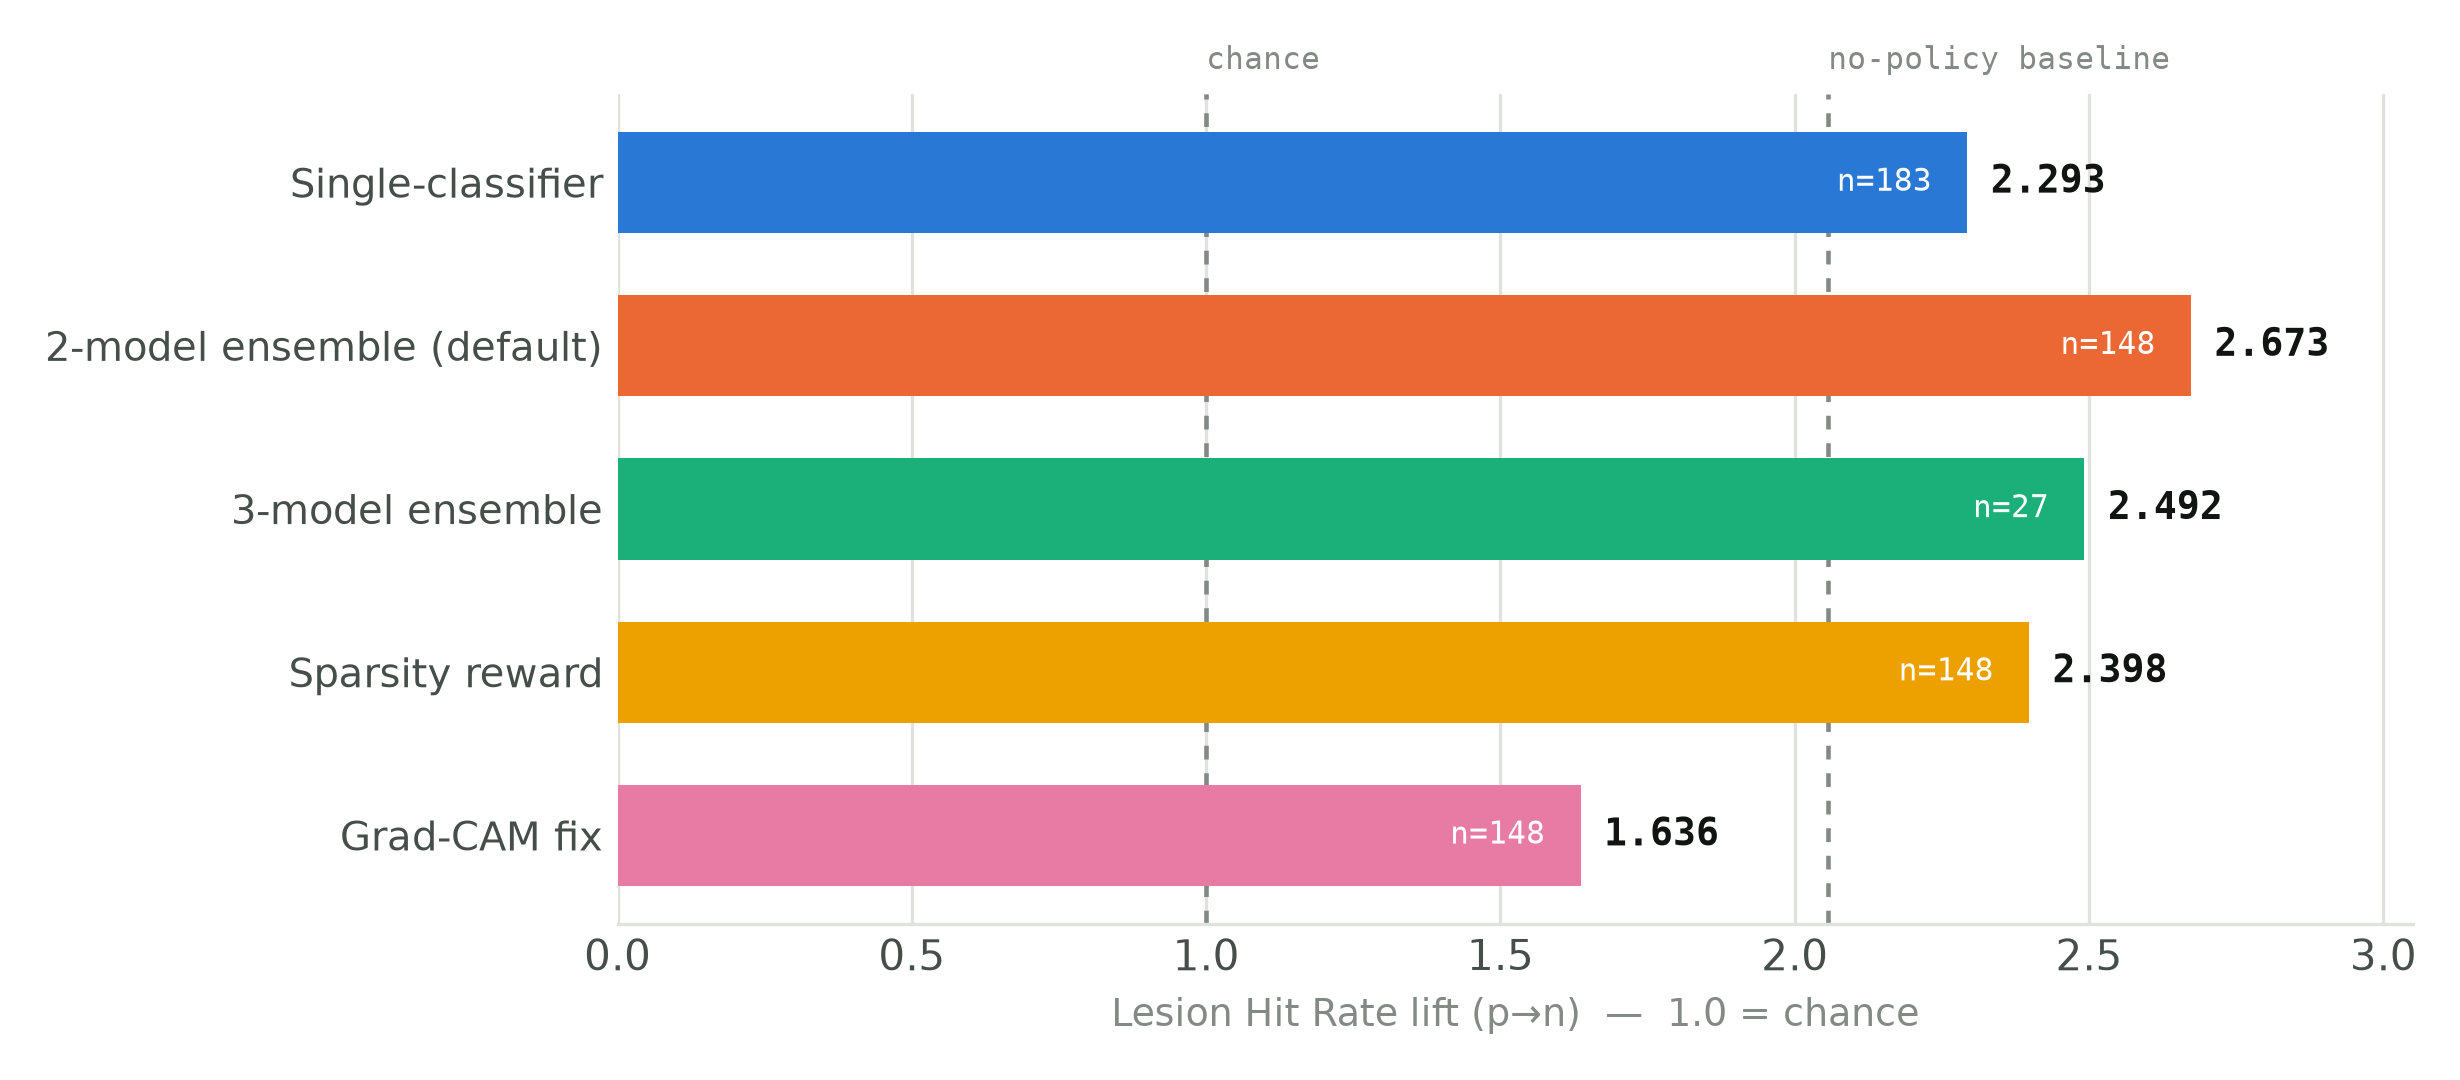
\includegraphics[width=0.9\linewidth]{figures/fig1_lhr_lift.png}
\caption{LHR lift (p$\to$n) across all five trained arms. Dashed lines mark chance (1.0) and the no-policy baseline. The no-policy arm under the same classifier-threshold grouping as the trained arms scores 2.046; the line is drawn at the no-policy value under the label protocol (groups selected by ground-truth label rather than classifier confidence), 2.057, which is indistinguishable at this scale.}
\label{fig:lhr-lift}
\end{figure}

\subsection{Five trained arms}
\label{sec:five-arms}

Every arm in Table~\ref{tab:five-arms} is a policy trained for 800 episodes per direction and evaluated end-to-end, with one training run per arm; none is a cheaper no-policy sweep or an offline proxy. The single-classifier arm predates the split and seeding controls of \S\ref{sec:controls} and was re-scored with corrected code, so its comparisons with the other four arms are not under an identical protocol. LHR verdicts are paired significance tests on the images two arms share, never differences of group means; transfer comparisons use each arm's own bootstrap CI (\S\ref{sec:cv-overstates}).

\paragraph{The ensemble-guided policy beats the single-classifier one, but the comparison is confounded.} Between trained policies, the single-classifier$\to$2-model step rests on a single run per arm: on the 76 shared annotated images the paired LHR-lift test favours the ensemble-guided policy ($d=0.482$, $p=7.1\times10^{-5}$). The two policies differ in more than guidance. The single-classifier policy predates the split and seeding controls, and probably also differs in reward weights, $a_1$ range and background-lock anchoring (\S\ref{sec:controls}; unverified), so this gap cannot be attributed to ensembling alone.
% TODO: single-classifier arm's training config not recorded; differences inferred from development history
Evidence on ensembling itself comes only from a policy-free sweep (three seeds; raw outputs were not preserved): generating without a policy under the label protocol, ensemble guidance raises paired per-image LHR lift over the no-countermeasure baseline by $+0.0694$ ($d=0.221$), $+0.0693$ ($d=0.223$) and $+0.0575$ ($d=0.151$) across three seeds, all with 95\% CIs excluding zero. That effect ($\approx+0.07$) is smaller than the trained comparison and is not a replication of it. Growing the ensemble to three members improves \texttt{pc} n$\to$p transfer from 0.462 to 0.623 with non-overlapping CIs and does not resolve on LHR ($n=12$, paired CI $[-0.298, +0.482]$), so we cannot say whether transfer and lesion targeting dissociate. It also moves \texttt{nih} in the right direction on both counts without separating from noise, and lowers mean CV further to 0.624 (0.685 n$\to$p, 0.563 p$\to$n).

\paragraph{The single-classifier policy beats a random one, but barely.} This comparison is measured against the single-classifier policy ($n=183$ annotated images), not the committed ensemble. Against the random-action arm on the same 183 images: paired lift difference $+0.090$ (95\% CI $[+0.021, +0.160]$), $t=2.551$, $p=0.0116$, Wilcoxon $p=0.0147$, $d=0.189$, trained better on 105/183. The effect is real but small, and considerably smaller than either negative result below.

\subsection{Two negative results}
\label{sec:negative-results}

\paragraph{An annealed sparsity reward fails at its own objective.} Edit concentration has stayed in the 0.21--0.32 band in every arm we measure. The sparsity term was built to address this and had been disabled throughout, leaving its annealing ramp inert. Enabled and isolated against the default, with $\lambda_{\text{sparsity}}$ configured to ramp to its target, concentration moved by less than 0.02 and the n$\to$p fraction of pixels changed went from 0.650 to 0.661. Meanwhile a paired test on the 148 shared annotated images gives a lift gap of $+0.275$ favouring the arm \emph{without} it (95\% CI $[+0.188, +0.363]$, $t=6.229$, $p=4.7\times10^{-9}$, $d=0.512$), and p$\to$n transfer falls from 0.293 to 0.212 with non-overlapping CIs on two of three validators. Without a working spatial mask the term degrades to plain unweighted $L_1$, which discourages edit mass uniformly rather than off-target mass specifically. This is a plausible account of why it competes with precise editing while failing at its own goal.

\paragraph{A Grad-CAM spatial constraint collapses the base task.} In a policy-free sweep (no trained policy), constraining edits to a Grad-CAM~\cite{selvaraju2017gradcam} region lowered LHR lift rather than raising it, so we diagnosed it directly. Scoring 263 member-image observations under the exact ensemble Grad-CAM path used during training contradicted the explanation on record: it is \texttt{chex}, not \texttt{rsna}, that degenerates (66/263, 25.1\% vs.\ 1/263), and it does so concentrated at \emph{low} predicted probability rather than near 0.5, which is consistent with output saturation zeroing the gradient. When \texttt{chex} degenerates the averaged mask falls back toward the least-constrained member alone, and CAM--lesion overlap falls with it (2.052, $n=127$ on clean episodes vs.\ 1.347, $n=23$ on partially degenerate ones). The remedy on record, a finer target layer, does eliminate the degeneracy (0\%/0.4\%) but drops baseline CAM--lesion lift to 1.196, barely above chance.

A policy trained under that remedy moved in the same direction, by a larger margin: CV collapses from 0.838 to 0.017, the paired LHR gap is $+1.037$ favouring the unconstrained arm (95\% CI $[+0.900, +1.178]$, $t=14.660$, $p=1.5\times10^{-30}$, $d=1.205$, better on 141/148 images), and transfer falls across all three validators. This is the largest paired effect size we measure anywhere, and it is against a mechanism introduced specifically to help. Constraining the action space to a finer, less confident CAM region does not trade a degeneracy problem for a localisation problem; it makes the base task substantially harder and every dependent metric degrades with it.

\subsection{Clinical proxy metrics}
\label{sec:clinical-proxies}

% TODO: unverified -- CTR deltas/t/p (n->p, p->n) have no traceable source for committed run
% TODO: unverified -- SCP relative spread 0.19% has no traceable source for committed run
We also computed two clinical proxies under the committed configuration, the Cardio-Thoracic Ratio (CTR) and a costophrenic-recess score (SCP), each with a paired $t$-test on the real-to-counterfactual delta (full results in Supp.~Sec.~E2). CTR shifts by less than 0.01 in both directions, far below the metric's clinical resolution, consistent with a cardiac silhouette that lies largely outside the lung mask gating the edits. SCP is numerically degenerate in this configuration (relative spread 0.19\%), so neither proxy supports a clinical claim.

\subsection{Qualitative examples}
\label{sec:qualitative}

\begin{figure}[H]
\centering
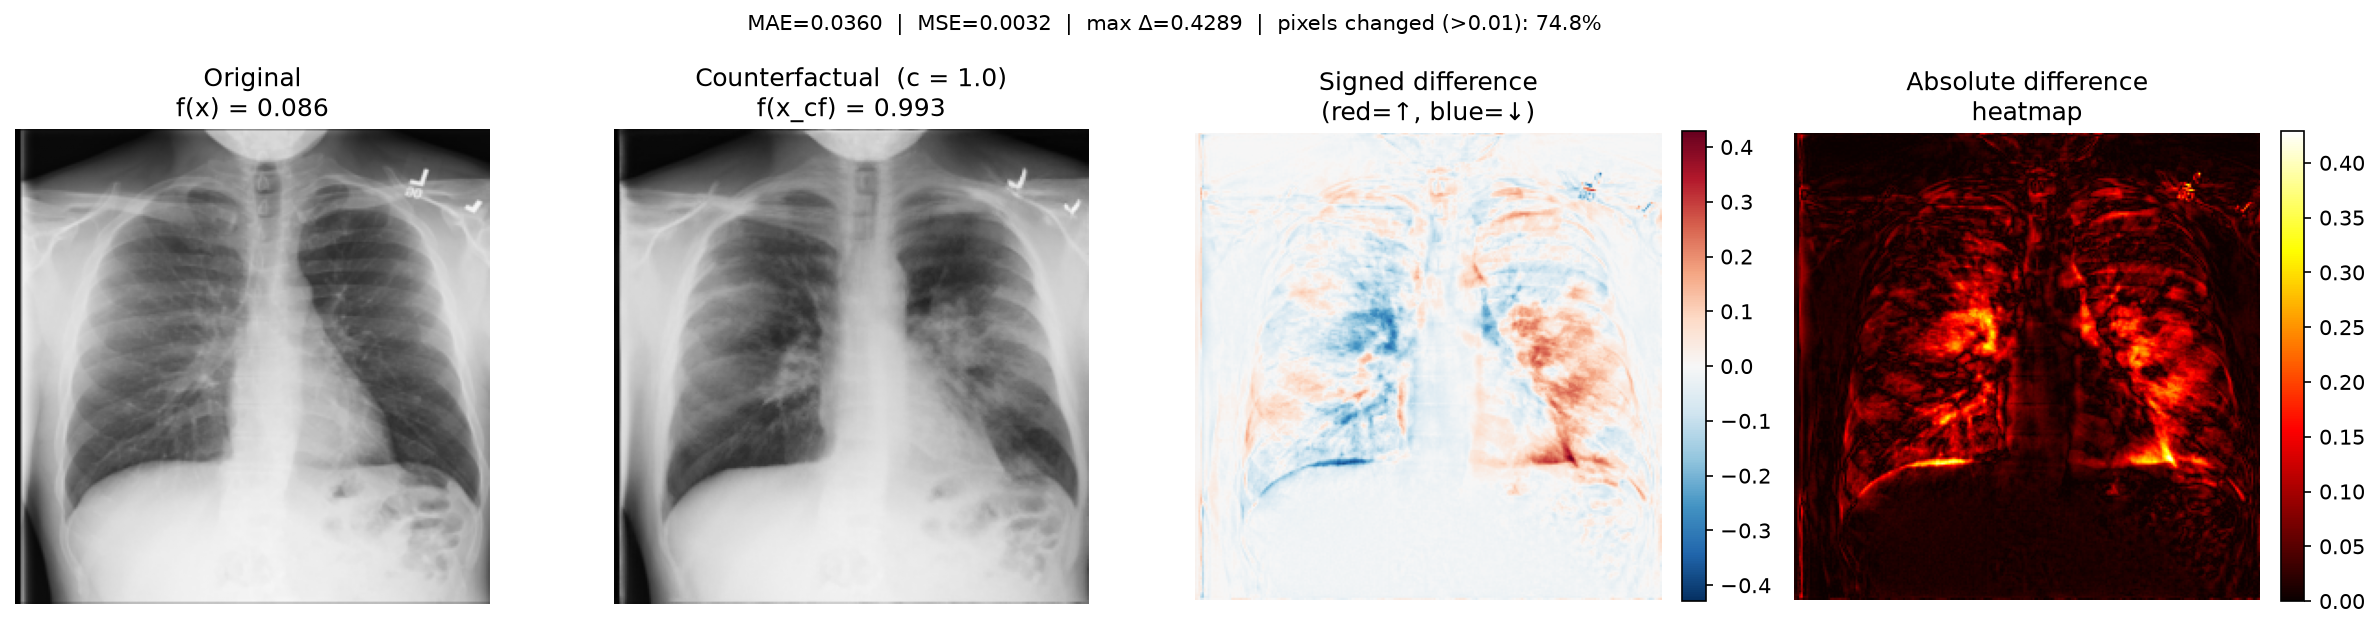
\includegraphics[width=0.9\linewidth]{figures/fig2_qualitative_np.png}
\caption{n$\to$p. Original, counterfactual, signed difference, absolute difference. Change is concentrated over the lung fields where an opacity is synthesized; anatomy outside the lung mask is largely retained, with smaller residual changes visible in the difference maps.}
\label{fig:qualitative-np}
\end{figure}

\begin{figure}[H]
\centering
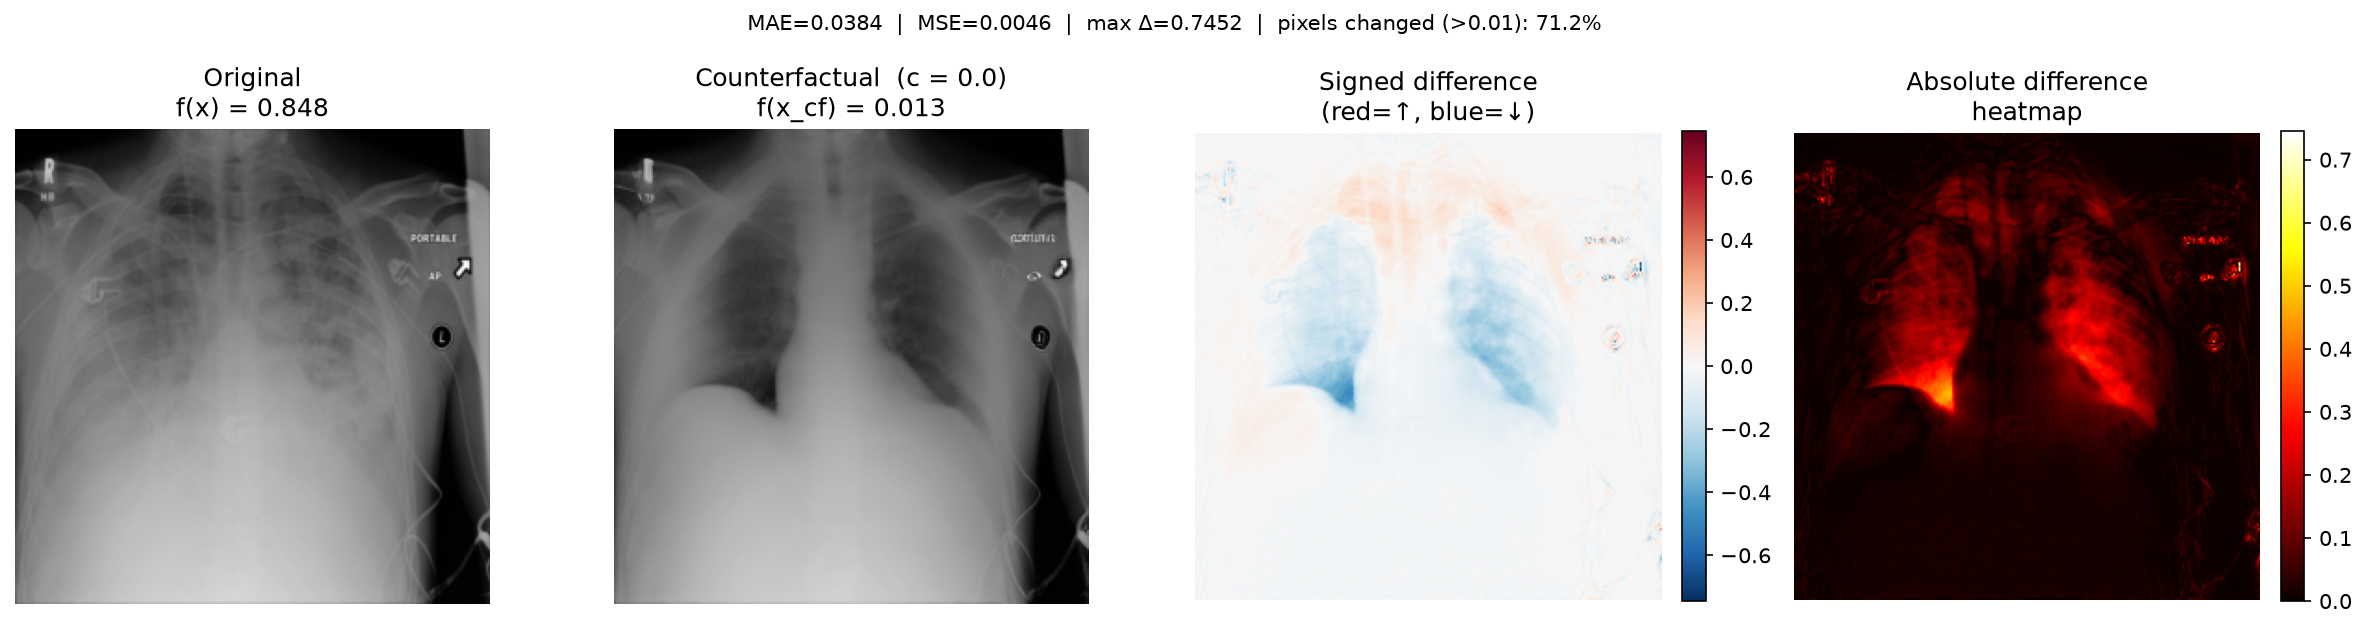
\includegraphics[width=0.9\linewidth]{figures/fig3_qualitative_pn.png}
\caption{p$\to$n. Original, counterfactual, signed difference, absolute difference. Change concentrates bilaterally over both lung fields, consistent with opacity removal, while gross anatomy and external hardware outside the lung mask remain visible, with smaller residual changes (including at the hardware) in the difference maps, consistent with a soft rather than exact lock.}
\label{fig:qualitative-pn}
\end{figure}

Figures~\ref{fig:qualitative-np} and~\ref{fig:qualitative-pn} show counterfactuals from the committed configuration, generated with each policy's mean action. In both, the guidance-classifier score crosses the CV margin ($f(x)=0.086 \to f(x_c)=0.993$ for n$\to$p; $0.848 \to 0.013$ for p$\to$n) while rib cage, mediastinal silhouette and external hardware remain visible outside the edited region; the difference maps still show smaller changes outside the lungs, including at the hardware, as expected from a soft lock. The p$\to$n edit is more concentrated than the n$\to$p one, but both remain diffuse relative to a lesion-shaped edit (\S\ref{sec:main-results}).
